\documentclass[12pt]{article}

\usepackage[margin=1in, left=1.3in]{geometry}

\usepackage{tocloft}
\renewcommand{\cftsecleader}{\cftdotfill{\cftdotsep}}


\usepackage{fancyhdr}
\pagestyle{fancy}
\fancyhf{}
\fancyfoot[C]{\thepage}
\renewcommand{\headrulewidth}{0.5pt}
\date{}

\usepackage{titlesec}
\titleformat{\section}
  {\normalfont\fontsize{14}{15}\bfseries}{\thesection}{0.5em}{}
  \titleformat{\subsection}
  {\normalfont\fontsize{12}{15}\bfseries}{\thesubsection}{0.5em}{}
   \titleformat{\subsubsection}
  {\normalfont\fontsize{12}{15}\bfseries}{\thesubsubsection}{0.5em}{}
  
  
\usepackage[labelfont=bf]{caption}
\captionsetup{labelfont=bf}


%\usepackage{epstopdf}
\usepackage{graphics}
\usepackage{graphicx}
\graphicspath{ {./Images/} }


\usepackage[nottoc]{tocbibind}


\begin{document}
% Title Page

\title{\textsc{\huge \bfseries High Security Automated Office}}

\clearpage\maketitle
\thispagestyle{empty}
\maketitle



\begin{center}


\emph{A Project Report Submitted 
on security and automation in a high secured office
 \\ for ALL INDIA RESEARCH CHAMPIONSHIPS 2018} \\[3cm]

\textsc{\bfseries By}\\[0.75cm]
KUMAR KUSHAGRA (it1725.iiitbhopal@gmail.com) \\
NAYAN VERMA (it1726.iiitbhopal@gmail.com)\\
K. SHARON (ec1747.iiitbhopal@gmail.com)\\


\vspace{3cm}
\textsc{\bfseries Under the supervision of}\\[0.75cm]

Mr. Saurabh Bharadwaj

\vspace{4.5cm}

\bfseries
Indian Institute of Information Technology Bhopal\\

\end{center}

\newpage
\clearpage
\pagenumbering{roman}
\setcounter{page}{1}
\thispagestyle{empty}
\fancyhead[L]{High Security Automated Office}
\tableofcontents


\newpage


\newpage
\listoffigures
\newpage
\clearpage
\setcounter{page}{1}
\pagenumbering{arabic}

\section{Introduction}
Our idea is to protect important documents and data by the help of mutual interaction between devices at any office place. Also by this we can avoid unnecessary entries towards sensitive places. Also we will guide the person who visits to room.  


\subsection{Abstract} 

We have a raspberry pie that will be connected to a camera, PIR sensors,mic ,magnetic lockers. As soon as someone approaches the door , the PIR sensors will detect his presence and the camera would start recording .After the person has entered the room the camera placed in the room will recognize his face from the data base .\\[0.3cm]
All the shelves, important devices and things will be shut by the raspberry pi ,only the devices and objects that the person is authorized to access will be available to him. Through the help of mic and speakers the raspberry pi would interact with the person and will guide him. The record of objects the person took or kept would be updated in a data base. We can work on many situations that are mentioned in the explanation. 

\subsection{Components Required}
\begin{table}[!h]
	\renewcommand{\arraystretch}{1.3}
	\caption{Name of Table}
	\label{table1}
	\centering
	\begin{tabular}{|c|c|c|c|}
		\hline
		\bfseries S No & \bfseries Components & \bfseries Quantity & \bfseries Cost(approx.)\\
		\hline
		1. & Raspberry Pi & 1 & Rs 3500\\
		\hline
		2. & Camera & 1 & Rs 1000\\
		\hline
		3. & PIR Sensors & 2 & Rs 100\\
		\hline
		4. & Mic & 1 & Rs 250\\
		\hline
		5.  & Hard Disk & 1 & Rs 3000(As per memory requirement)\\
		\hline
		6. & Speakers & 1 & Rs 500\\
		\hline
		7. & Memory Card & 1 & Rs 400\\
		\hline
		8. & LEDs & 10 & Rs 5\\
		\hline
		9. & Relay & 4 & Rs 250\\
		\hline
		10. &  Magnetic Door Locker & 3 & Rs 1500\\
		\hline
				
	\end{tabular}
\end{table}
Total Cost(approx.)= Rs 12,000

\newpage
\section{Explanation}
Whenever a person visits the room , then camera will recognize the face and evaluate whether the person is allowed to access the documents kept in the room or not. As soon as he enters, the doors will get locked so that no one else can visit and do any harm to anything. Also the cameras will start recording just to monitor his activities.\\[0.5cm]


\begin{figure}[!h]
	\centering
	{
		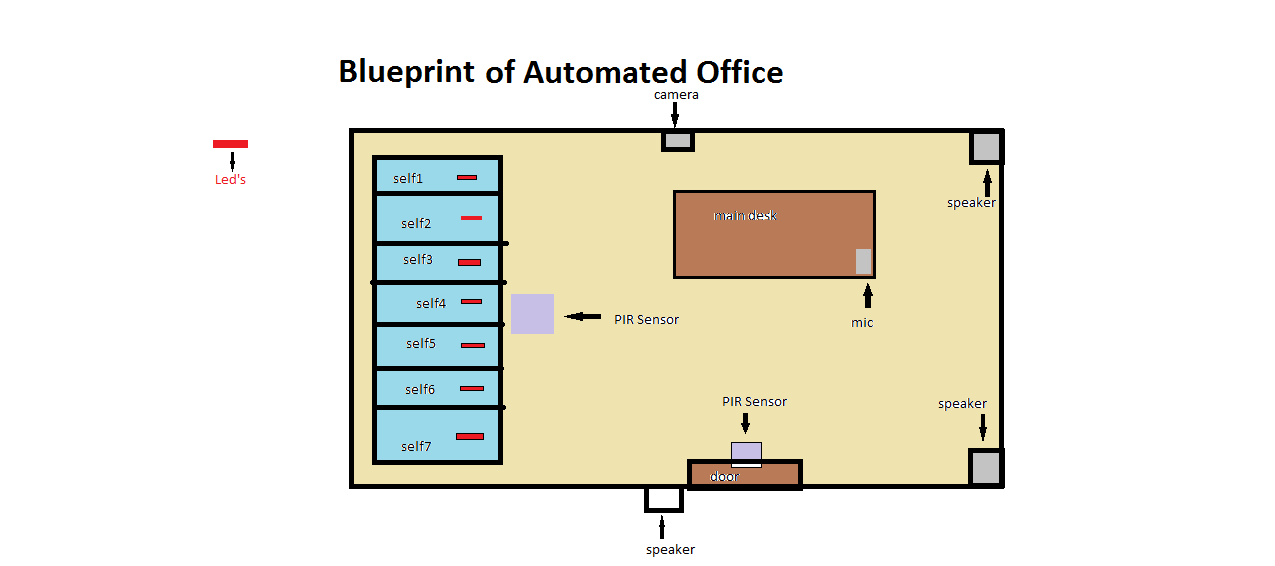
\includegraphics[width=5in]{main_room.png}
	}
	\caption{Blueprint of the Room}
	\label{Figure1}
\end{figure}


\subsection{Case 1}
If the person visited has the access to given room then we will welcome him and ask his purpose of visit. Then he will come near to the mic and tell us his purpose.

\subsubsection{Needs document}
If he will be needing some physical document then we will ask him about that. Whatever he will say we will read it and accordingly we will instruct him which shelf he has to go and we will unlock that shelf too. Also we will blink the led of shelf so that he can visit over there. As soon as he visits near to that shelf, then that led will stop blinking. We will be doing this with the help of a PIR Sensor. Also when he will move away from the shelf after completing his task then the shelf will automatically get locked .If the file has been taken by someone else ,we would tell his name and designation or any other necessary detail to that person . After this we will ask him whether he has some more work to do or not?? If the answer is yes, the same things will continue else the door will get open and he can leave the room .Our raspberry pi will store all the records who has taken which file, when have they taken it etc. As the door get closed then the camera will monitor for few more seconds and shut down if no one is in the room now ,if someone is still in the room then our raspberry pi will interact with him.
   
\subsubsection{Needs data from computer}
If he need some files stored in a computer or laptop then he would need to speak the name of the file in our mic , our program in the raspberry pi will convert the speech into text and search the file in the laptop or computer.Our raspberry pi will check if the person is permitted to access the file or not.If permitted the person will now have to insert a pen-drive in the computer .Our program will now copy that file to the pen-drive , and a message saying "done" will be said by the speaker , if the file is not found then an error statement will be conveyed to the person .The inputs of the computer or the laptop like keyboard or mouse , will be inactive during this period. This will make the sensitive data in the computer or laptop more secure .After the work is done we would ask the person if we could do something else for him , if he answers no then door lock would open and the person can go out.      

\subsubsection{Return document}
In this he will tell us his purpose of his visit, If he is there to return some documents then we will ask him the name of the file he wish to return, our program in the raspberry pi will search in the database the right location of the document and the LED of that shelf will start blinking .The shelf will be unlocked and the person can return the file . After this we will ask him whether he has some more work to do or not?? If the answer is yes, the same things will continue else the door will get open and he can leave the room .Our raspberry pi will update the records who has taken which file, when have they taken it , when they returned it etc. As the door get closed then the camera will monitor for few more seconds and shut down if no one is in the room now ,if someone is still in the room then our raspberry pi will interact with him.

\subsection{Case 2}
If our system does not recognize the person then the control room will be informed and his actions will be monitored , we will ask some general questions like his name , the purpose of his visit. 

\subsubsection{Give permission}
As he is monitored and the control room give him the permission to access then he can work normally , our raspberry pi will store his photo ,name etc information in the data base for future reference.

\subsubsection{Permission denied}
If the control room denies the permission to the person then the raspberry pi will apologize and ask him to leave the room .All the shelves will remain locked , the laptop or the computer .If the person will not leave the room within some time or come close to any ot the laptop, computer or shelves , the control room will be alerted and the gate will be locked so that we can trap him.  

\subsection{Case 3}
If more then one person enters and one is authorized and the others are not, then our system will first ask for the details of those people and once the authorized person conforms that they are his responsibility then we will also give him the access for that particular period.

\subsection{Case 4}
When the room is already occupied by someone inside ,we will ask the person outside the room to wait through a speaker placed outside the room.\\[1cm] 


\begin{figure}[!h]
	\centering
	{
		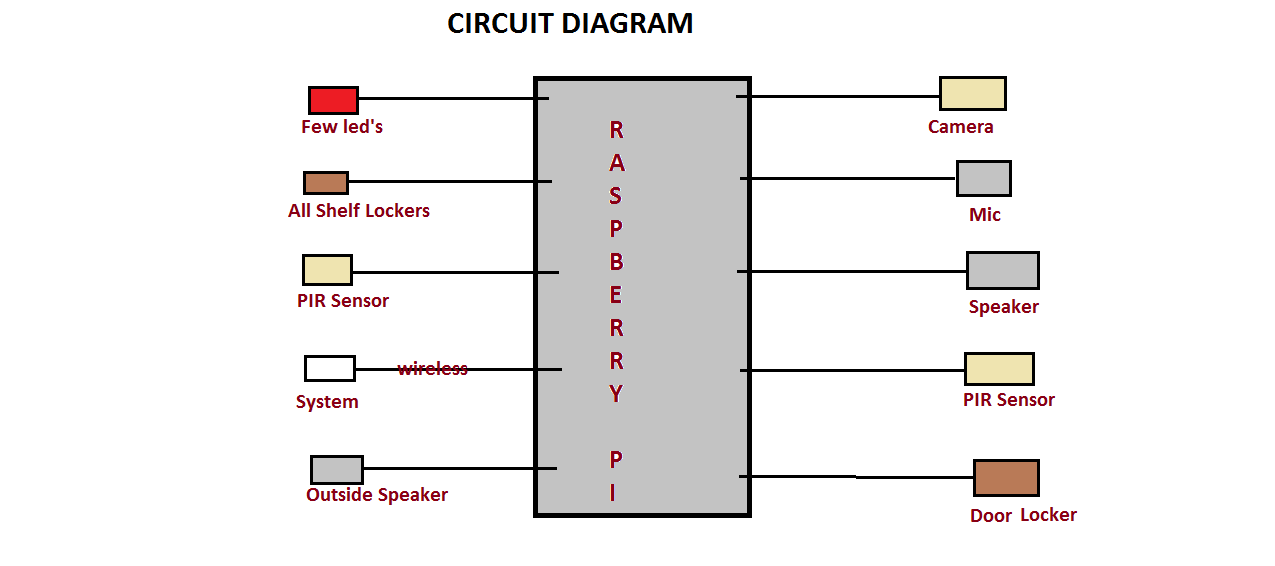
\includegraphics[width=5in]{circuit_diagram.png}
	}
	\caption{Circuit Diagram}
	\label{Figure1}
\end{figure}

\newpage
\section{Features}
Our project has the following features :-\\[0.5cm]
1. Less human effort and more security.\\[0.2cm]
2. A high security room which gives 24/7 access to all people with a trap for unauthorized people.\\[0.2cm]
3. Less memory space required as only the important recordings will be stored.\\[0.2cm]
4. Provide help to people in finding what they need.\\[0.2cm]
5. It maintains the record of no. of times the document excessed and by whom.\\



\section{Further Applications}
Our project can be modified a little and be useful in many other places like :-
 
\subsection{Locker Room}
Our model can be very handy and efficient in the locker rooms .It gives people more privacy to its customers also only few people can have access to it .Even if you are having the keys of your locker ,still you can't open it if the main owner doesn't provide you with its access.Also it makes our locker room more safer from any mischievous activity as the person can get locked inside and the security will get informed. 
 
\subsection{Police Station}
It is always heard that misleading happens with the evidences at police stations which may lead to injustice .Our model will keep all the records of every file and its location . 

\subsection{Dispensary}
With the help of our model we can make an automated dispensary where people has to enter the medicines required by them in a system and can do the payment there by card. Once they pay for their medicine they will be instructed where it is kept, so that they can go and collect it. Also by this we can maintain a proper data of medicines available and used.

\subsection{Other Important Places}
We can also implement it at some other places where we want to have surveillance as we might have something precious kept over there. The places may be house,exam rooms(where we keep answer sheets and exam papers),jewelery stores etc. 

\end{document}